\documentclass[tikz,border=10pt]{standalone}
\usepackage{tikz}
\usetikzlibrary{matrix}

\tikzset{
  tablecell/.style={draw=black!70, line width=1.0pt, minimum width=3.2cm, minimum height=0.95cm, align=center, text width=3.0cm, fill=none},
  headcell/.style={tablecell, draw=blue!70!black, line width=1.2pt},
  leftcell/.style={tablecell, draw=green!50!black, line width=1.2pt}
}

\begin{document}
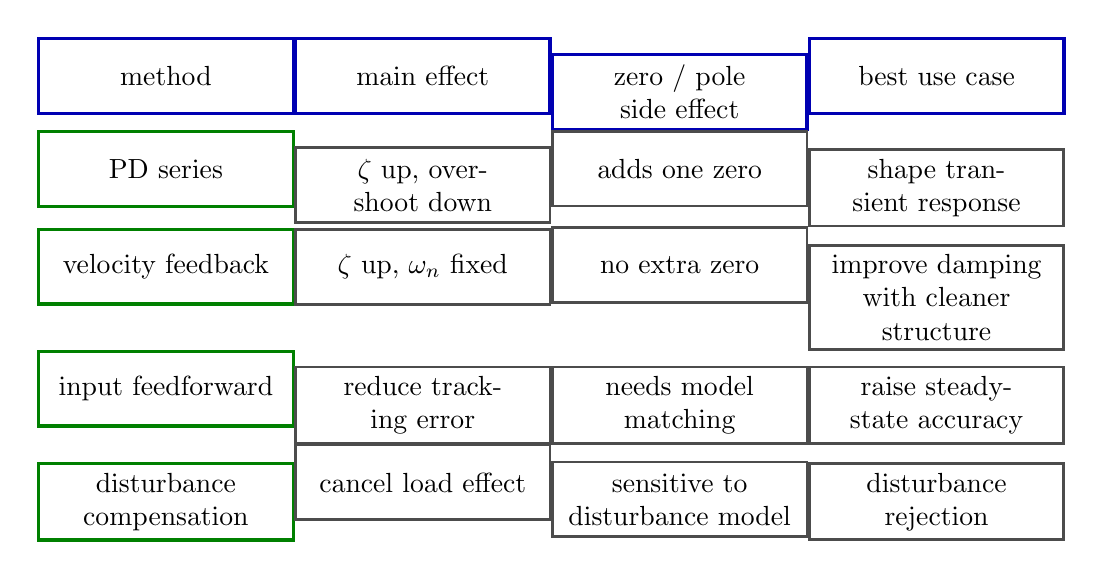
\begin{tikzpicture}
  \matrix[matrix of nodes, nodes in empty cells, row sep=-\pgflinewidth, column sep=-\pgflinewidth] {
    \node[headcell] {method}; &
    \node[headcell] {main effect}; &
    \node[headcell] {zero / pole side effect}; &
    \node[headcell] {best use case}; \\
    \node[leftcell] {PD series}; &
    \node[tablecell] {$\zeta$ up, overshoot down}; &
    \node[tablecell] {adds one zero}; &
    \node[tablecell] {shape transient response}; \\
    \node[leftcell] {velocity feedback}; &
    \node[tablecell] {$\zeta$ up, $\omega_n$ fixed}; &
    \node[tablecell] {no extra zero}; &
    \node[tablecell] {improve damping with cleaner structure}; \\
    \node[leftcell] {input feedforward}; &
    \node[tablecell] {reduce tracking error}; &
    \node[tablecell] {needs model matching}; &
    \node[tablecell] {raise steady-state accuracy}; \\
    \node[leftcell] {disturbance compensation}; &
    \node[tablecell] {cancel load effect}; &
    \node[tablecell] {sensitive to disturbance model}; &
    \node[tablecell] {disturbance rejection}; \\
  };
\end{tikzpicture}
\end{document}
